% Options for packages loaded elsewhere
\PassOptionsToPackage{unicode}{hyperref}
\PassOptionsToPackage{hyphens}{url}
\PassOptionsToPackage{dvipsnames,svgnames,x11names}{xcolor}
%
\documentclass[
  12pt,
  letterpaper,
  DIV=11,
  numbers=noendperiod,
  twoside]{scrreprt}

\usepackage{amsmath,amssymb}
\usepackage{iftex}
\ifPDFTeX
  \usepackage[T1]{fontenc}
  \usepackage[utf8]{inputenc}
  \usepackage{textcomp} % provide euro and other symbols
\else % if luatex or xetex
  \usepackage{unicode-math}
  \defaultfontfeatures{Scale=MatchLowercase}
  \defaultfontfeatures[\rmfamily]{Ligatures=TeX,Scale=1}
\fi
\usepackage[]{libertinus}
\ifPDFTeX\else  
    % xetex/luatex font selection
\fi
% Use upquote if available, for straight quotes in verbatim environments
\IfFileExists{upquote.sty}{\usepackage{upquote}}{}
\IfFileExists{microtype.sty}{% use microtype if available
  \usepackage[]{microtype}
  \UseMicrotypeSet[protrusion]{basicmath} % disable protrusion for tt fonts
}{}
\makeatletter
\@ifundefined{KOMAClassName}{% if non-KOMA class
  \IfFileExists{parskip.sty}{%
    \usepackage{parskip}
  }{% else
    \setlength{\parindent}{0pt}
    \setlength{\parskip}{6pt plus 2pt minus 1pt}}
}{% if KOMA class
  \KOMAoptions{parskip=half}}
\makeatother
\usepackage{xcolor}
\usepackage[paperwidth=890pt,paperheight=890pt,left=30pt,textwidth=500pt,marginparsep=30pt,marginparwidth=300pt,top=50pt,bottom=50pt,heightrounded]{geometry}
\setlength{\emergencystretch}{3em} % prevent overfull lines
\setcounter{secnumdepth}{5}
% Make \paragraph and \subparagraph free-standing
\ifx\paragraph\undefined\else
  \let\oldparagraph\paragraph
  \renewcommand{\paragraph}[1]{\oldparagraph{#1}\mbox{}}
\fi
\ifx\subparagraph\undefined\else
  \let\oldsubparagraph\subparagraph
  \renewcommand{\subparagraph}[1]{\oldsubparagraph{#1}\mbox{}}
\fi


\providecommand{\tightlist}{%
  \setlength{\itemsep}{0pt}\setlength{\parskip}{0pt}}\usepackage{longtable,booktabs,array}
\usepackage{calc} % for calculating minipage widths
% Correct order of tables after \paragraph or \subparagraph
\usepackage{etoolbox}
\makeatletter
\patchcmd\longtable{\par}{\if@noskipsec\mbox{}\fi\par}{}{}
\makeatother
% Allow footnotes in longtable head/foot
\IfFileExists{footnotehyper.sty}{\usepackage{footnotehyper}}{\usepackage{footnote}}
\makesavenoteenv{longtable}
\usepackage{graphicx}
\makeatletter
\def\maxwidth{\ifdim\Gin@nat@width>\linewidth\linewidth\else\Gin@nat@width\fi}
\def\maxheight{\ifdim\Gin@nat@height>\textheight\textheight\else\Gin@nat@height\fi}
\makeatother
% Scale images if necessary, so that they will not overflow the page
% margins by default, and it is still possible to overwrite the defaults
% using explicit options in \includegraphics[width, height, ...]{}
\setkeys{Gin}{width=\maxwidth,height=\maxheight,keepaspectratio}
% Set default figure placement to htbp
\makeatletter
\def\fps@figure{htbp}
\makeatother
% definitions for citeproc citations
\NewDocumentCommand\citeproctext{}{}
\NewDocumentCommand\citeproc{mm}{%
  \begingroup\def\citeproctext{#2}\cite{#1}\endgroup}
\makeatletter
 % allow citations to break across lines
 \let\@cite@ofmt\@firstofone
 % avoid brackets around text for \cite:
 \def\@biblabel#1{}
 \def\@cite#1#2{{#1\if@tempswa , #2\fi}}
\makeatother
\newlength{\cslhangindent}
\setlength{\cslhangindent}{1.5em}
\newlength{\csllabelwidth}
\setlength{\csllabelwidth}{3em}
\newenvironment{CSLReferences}[2] % #1 hanging-indent, #2 entry-spacing
 {\begin{list}{}{%
  \setlength{\itemindent}{0pt}
  \setlength{\leftmargin}{0pt}
  \setlength{\parsep}{0pt}
  % turn on hanging indent if param 1 is 1
  \ifodd #1
   \setlength{\leftmargin}{\cslhangindent}
   \setlength{\itemindent}{-1\cslhangindent}
  \fi
  % set entry spacing
  \setlength{\itemsep}{#2\baselineskip}}}
 {\end{list}}
\usepackage{calc}
\newcommand{\CSLBlock}[1]{\hfill\break\parbox[t]{\linewidth}{\strut\ignorespaces#1\strut}}
\newcommand{\CSLLeftMargin}[1]{\parbox[t]{\csllabelwidth}{\strut#1\strut}}
\newcommand{\CSLRightInline}[1]{\parbox[t]{\linewidth - \csllabelwidth}{\strut#1\strut}}
\newcommand{\CSLIndent}[1]{\hspace{\cslhangindent}#1}

\usepackage{marginfix}[=1.2]
\usepackage{sidenotes}

\usepackage{xeCJK}
\usepackage{fontspec}
% \renewcommand\allcapsspacing[1]{{\addfontfeature{LetterSpace=15}#1}}
% \renewcommand\smallcapsspacing[1]{{\addfontfeature{LetterSpace=10}#1}}

\usepackage{amssymb}
\usepackage{amsthm}
\usepackage{amsmath}
\usepackage{amsfonts}
\usepackage{unicode-math}
\usepackage{mathtools}
\usepackage{mathrsfs}

\usepackage{qrcode}
\usepackage{xcolor}
\usepackage{relsize}
\usepackage{soul}
% \usepackage{caption}

\usepackage{tikz-cd}
\usepackage{quiver}
\usepackage{frege}
\usepackage{empheq}

\newcommand{\ourblue}{\color[RGB]{0, 32, 96}}
\usetikzlibrary{fit}
\newenvironment{dummyenv}{}{}
\newcommand{\class}[2]{}
\newcommand{\cssId}[2]{}

\let\linebreakto\linebreak
\renewcommand{\linebreak}{}
\let\captionto\caption
\let\captionsetupto\captionsetup
\let\labelitemito\labelitemi
\let\phantomsectionto\phantomsection
% \let\textfloatsepto\textfloatsep
% \let\floatsepto\floatsep
% \let\intextsepto\intextsep
\counterwithout{footnote}{chapter}

\usepackage{graphicx} % allow embedded images
  \setkeys{Gin}{width=\linewidth,totalheight=\textheight,keepaspectratio}
%   \graphicspath{{graphics/}} % set of paths to search for images

\usepackage{booktabs} % book-quality tables 
\usepackage{units}    % non-stacked fractions and better unit spacing
\usepackage{multicol} % multiple column layout facilities
\usepackage{lipsum}   % filler text
\usepackage{array}
\usepackage{fancyvrb} % extended verbatim environments
  \fvset{fontsize=\normalsize}% default font size for fancy-verbatim environments
\usepackage{hyperref}

\usepackage{fancyhdr}
\renewcommand{\headrulewidth}{0pt}
\setlength{\headwidth}{820pt}
\pagestyle{fancy}
\fancyhf{}
\cfoot{}\lfoot{}\rfoot{}
\fancyhead{}
\fancyfoot{}
\fancyhf{}
\fancyhead[RO,LE]{\thepage}
\usepackage{datetime}
\usepackage{pgfplots}
\usepackage[super]{nth}

% TODO?
% \usepackage{quiver}

\pgfplotsset{compat=1.17}
\usetikzlibrary{intersections,angles,quotes}
\usepgfplotslibrary{fillbetween}

\def\mathnote#1{%
  \tag*{\rlap{\hspace\marginparsep{\parbox[t]{\marginparwidth}{\footnotesize#1}}}}%
}
\def\mathnotes#1{%
  \tag*{\rlap{\hspace\marginparsep\smash{\parbox[t]{\marginparwidth}{\footnotesize#1}}}}%
}
\def\mathnoteps#1{%
  \tag*{\rlap{\hspace\marginparsep{\parbox[t]{\marginparwidth}{\footnotesize#1}}}}%
}

\extrafloats{100}

\usepackage{ifoddpage}
\newcommand{\oddorevenarrow}{
  \checkoddpage
  \ifoddpage
    \leftarrow
  \else
    \rightarrow
  \fi
}
\KOMAoption{captions}{tableheading}
\makeatletter
\@ifpackageloaded{float}{}{\usepackage{float}}
\floatstyle{plain}
\@ifundefined{c@chapter}{\newfloat{eqnc}{h}{loeqn}}{\newfloat{eqnc}{h}{loeqn}[chapter]}
\floatname{eqnc}{}
\newcommand*\listofeqncs{\listof{eqnc}{List of s}}
\makeatother
\makeatletter
\@ifpackageloaded{float}{}{\usepackage{float}}
\floatstyle{plain}
\@ifundefined{c@chapter}{\newfloat{plst}{h}{loplst}}{\newfloat{plst}{h}{loplst}[chapter]}
\floatname{plst}{Proof Listing}
\newcommand*\listofplsts{\listof{plst}{List of Proof Listings}}
\makeatother
\makeatletter
\@ifpackageloaded{tcolorbox}{}{\usepackage[skins,breakable]{tcolorbox}}
\@ifpackageloaded{fontawesome5}{}{\usepackage{fontawesome5}}
\definecolor{quarto-callout-color}{HTML}{909090}
\definecolor{quarto-callout-note-color}{HTML}{0758E5}
\definecolor{quarto-callout-important-color}{HTML}{CC1914}
\definecolor{quarto-callout-warning-color}{HTML}{EB9113}
\definecolor{quarto-callout-tip-color}{HTML}{00A047}
\definecolor{quarto-callout-caution-color}{HTML}{FC5300}
\definecolor{quarto-callout-color-frame}{HTML}{acacac}
\definecolor{quarto-callout-note-color-frame}{HTML}{4582ec}
\definecolor{quarto-callout-important-color-frame}{HTML}{d9534f}
\definecolor{quarto-callout-warning-color-frame}{HTML}{f0ad4e}
\definecolor{quarto-callout-tip-color-frame}{HTML}{02b875}
\definecolor{quarto-callout-caution-color-frame}{HTML}{fd7e14}
\makeatother
\makeatletter
\@ifpackageloaded{bookmark}{}{\usepackage{bookmark}}
\makeatother
\makeatletter
\@ifpackageloaded{caption}{}{\usepackage{caption}}
\AtBeginDocument{%
\ifdefined\contentsname
  \renewcommand*\contentsname{Table of contents}
\else
  \newcommand\contentsname{Table of contents}
\fi
\ifdefined\listfigurename
  \renewcommand*\listfigurename{List of Figures}
\else
  \newcommand\listfigurename{List of Figures}
\fi
\ifdefined\listtablename
  \renewcommand*\listtablename{List of Tables}
\else
  \newcommand\listtablename{List of Tables}
\fi
\ifdefined\figurename
  \renewcommand*\figurename{Figure}
\else
  \newcommand\figurename{Figure}
\fi
\ifdefined\tablename
  \renewcommand*\tablename{Table}
\else
  \newcommand\tablename{Table}
\fi
}
\@ifpackageloaded{float}{}{\usepackage{float}}
\floatstyle{ruled}
\@ifundefined{c@chapter}{\newfloat{codelisting}{h}{lop}}{\newfloat{codelisting}{h}{lop}[chapter]}
\floatname{codelisting}{Listing}
\newcommand*\listoflistings{\listof{codelisting}{List of Listings}}
\usepackage{amsthm}
\theoremstyle{remark}
\AtBeginDocument{\renewcommand*{\proofname}{Proof}}
\newtheorem*{remark}{Remark}
\newtheorem*{solution}{Solution}
\newtheorem{refremark}{Remark}[chapter]
\newtheorem{refsolution}{Solution}[chapter]
\makeatother
\makeatletter
\makeatother
\makeatletter
\@ifpackageloaded{caption}{}{\usepackage{caption}}
\@ifpackageloaded{subcaption}{}{\usepackage{subcaption}}
\makeatother
\makeatletter
\@ifpackageloaded{sidenotes}{}{\usepackage{sidenotes}}
\@ifpackageloaded{marginnote}{}{\usepackage{marginnote}}
\makeatother
\ifLuaTeX
  \usepackage{selnolig}  % disable illegal ligatures
\fi
\usepackage{bookmark}

\IfFileExists{xurl.sty}{\usepackage{xurl}}{} % add URL line breaks if available
\urlstyle{same} % disable monospaced font for URLs
\hypersetup{
  pdftitle={Gödelian Explorations},
  pdfauthor={Gary Mar},
  colorlinks=true,
  linkcolor={blue},
  filecolor={Maroon},
  citecolor={Blue},
  urlcolor={Blue},
  pdfcreator={LaTeX via pandoc}}

\title{Gödelian Explorations}
\author{Gary Mar}
\date{2030-01-01}

\begin{document}
\maketitle

\renewcommand\phantomsection{}
% \setlength{\floatsep}{0pt}
% \setlength{\textfloatsep}{0pt}
% \setlength{\intextsep}{0pt}
\floatplacement{eqnc}{H}

% \renewcommand{\captionsetup}{}
% \renewcommand{\caption}[1]{#1}

\newlength{\parskipto}
\setlength{\parskipto}{\parskip}

\setlength{\floatsep}{0cm}
\setlength{\textfloatsep}{0cm}
\setlength{\intextsep}{0cm}

\setmathfont{TeX Gyre Termes Math}[range=\smwhtdiamond]
\setmathfont{LibertinusMath-Regular.otf}[range=]

\renewcommand*\contentsname{Table of contents}
{
\hypersetup{linkcolor=}
\setcounter{tocdepth}{2}
\tableofcontents
}
\bookmarksetup{startatroot}

\chapter*{Preface}\label{preface}
\addcontentsline{toc}{chapter}{Preface}

\markboth{Preface}{Preface}

This is a Quarto book.

To learn more about Quarto books visit
\url{https://quarto.org/docs/books}.

\bookmarksetup{startatroot}

\chapter{`Must' and `Might' --- The Modal Logic of Necessity and
Possibility}\label{must-and-might-the-modal-logic-of-necessity-and-possibility}

\section{\texorpdfstring{\textsc{Modes of Truth and Modal
Logics}}{Modes of Truth and Modal Logics}}\label{modes-of-truth-and-modal-logics}

Historically, notions like \emph{necessity}, \emph{possibility},
\emph{impossibility}, and \emph{contingency} were thought of as modes of
truth or ways in which a proposition could be true or false. \emph{Modal
logic} began as the study of the logic of these modes of truth.

Aristotle, in Chapter 9 of \emph{De Interpretatione}, discusses modality
in his famous example of the sea battle. Suppose the sea battle will be
fought tomorrow. Then it was true yesterday that it would be fought
tomorrow. So if all past truths are necessarily true, then it is
necessarily true now that the battle will be fought tomorrow. A similar
argument holds on the supposition that the sea battle will not be fought
tomorrow. Aristotle proposed solving this problem of \emph{logical
fatalism} by denying that future contingent propositions have definite
truth-values.

Using the `\(\Box\)' for `it is necessary that', the principle that all
necessary truths are in fact
\begin{equation}\phantomsection\label{eq-modal-axiom-T}{
\Box \mathrm{P}\to \mathrm{P},\tag*{(\textbf{T})}
}\end{equation} but adding its converse that all truths are necessary
truths: \begin{equation}\phantomsection\label{eq-modal-axiom-V}{
\mathrm{P} \to \Box \mathrm{P} \tag*{(\textbf{V})}
}\end{equation} collapses the notions of truth and necessary truth.

Medieval philosophers, concerned with such theological issues as
articulating the nature of the Trinity, appealed to such modal notions
as essence and accident, contingency and necessity in their labyrinthine
theological reflections.\sidenote{\footnotesize The theological, if not the political,
  roots Great Schism of 1054, which can be traced back to a disagreement
  about the modalities of the Persons of the Trinity. The Nicean Creed
  (325) uses the term \emph{homoousios} (from the Greek \emph{homo} =
  `same` and \emph{ousios} = `essence' or `substance'), in contrast to
  \emph{homoiousios} (from the Greek \emph{homoi} = `similar') making
  the solitary \emph{i} the jot and tittle of Nicean Creedal Orthodoxy.
  The Greek Church preferred the latter term since the former had been
  used by the Syrian Bishop of Antioch to espouse \emph{modal
  monarchism}, the heresy that the Heavenly Father, Resurrected Son and
  Holy Spirit are not three distinct Persons, but are rather
  different~\emph{modes}~or~\emph{aspects}~of one monadic God perceived
  by believers as distinct persons. The Latin Church adopted the former
  siding with Athanasius against the heretic Arius, who denied that
  Jesus was co-equal and co-eternal with the Father. The Second Council
  of Nicea (381), among other changes, inserted the word \emph{filioque}
  (from the Latin \emph{filio} = the son, and \emph{que} = ``and'') into
  the Nicean-Constantinopolitan Creed and the Latin mass. In Latin
  theology, the three Persons of the Trinity are logically distinguished
  by the formal relations of ``proceeding from'' citing such proof texts
  as Phil. 1:9, Titus 3:6, Acts 2:33. Orthodox theology, citing the
  words of Jesus in proof texts such John 15:26, regarded the insertion
  of \emph{filioque} into the Nicean-Constantipolitan creed, is as
  Semi-Sabellianism. The great church historian Pelikan (1988: 90)
  opined: ``If there is a special circle of the inferno described by
  Dante reserved for historians of theology, the principal homework
  assigned to that subdivision of Hell for at least the first several
  eons of eternity may well be a thorough study of all the
  treatises\ldots{} devoted to the inquiry: Does the Holy Spirit proceed
  from the Father only, as Eastern Christendom contends, or from both
  the Father and the Son as the Latin Church teaches?'' In 1989 Pope
  John Paul II and Patriarch Demetrius knelt together in Rome and
  recited the Nicene Creed without the
  \emph{filioque}.\linebreak\linebreak
\begin{CSLReferences}{2}{0}
\bibitem[\citeproctext]{ref-Pelikan1988melody}
Pelikan, J. 1988. \emph{The melody of theology: A philosophical
dictionary}. Harvard University Press.
\end{CSLReferences}
\linebreak}
Akin to the problem is logical fatalism is the problem of
\emph{theological fatalism}: the problem of reconciling divine
foreknowledge and human freedom. Saint Augustine (354--430) in his
treatise \emph{On the Free Choice of Will} considers an argument for
\emph{theological fatalism} proposed by Evodius. Evodius argued that
``God foreknew that man would sin, that which God foreknew must
necessarily come to pass.'' We may set forth this argument for
theological fatalism for a particular case as follows:

\renewcommand\labelitemi{}

\begin{itemize}
\tightlist
\item
  If God knew that Adam would sin, then, necessarily Adam sinned.
\item
  God knew that Adam would sin (because God is omniscient).
\item
  Therefore, Adam necessarily sinned.
\end{itemize}

St.~Thomas Aquinas (1225--1274) in his \emph{Summa Contra Gentiles}
(part I, chapter 67) criticized this kind of argument as resting on an
amphiboly. The critical first premise ``if God knew Adam would sin,
then, \emph{necessarily}, Adam sinned'' is ambiguous between

\begin{itemize}
\tightlist
\item
  \phantomsection\label{eq-modal-1a}{(1\emph{a})} It is necessarily the
  case that if God knows that Adam will sin then Adam will sin.
\item
  \phantomsection\label{eq-modal-1b}{(1\emph{b})} If God knows that Adam
  will sin, then it is necessary that Adam will sin.
\end{itemize}

\renewcommand\labelitemi{\labelitemito}

Aquinas called \hyperref[eq-modal-1a]{(1\emph{a})} the \emph{necessity
of the consequence} contrasting it with
\hyperref[eq-modal-1b]{(1\emph{b})} the \emph{necessity of the
consequent}. Using the `\(\Box\)' to abbreviate `it is necessary that',
the difference between these two can be made more perspicuous with
symbols: \begin{equation}\phantomsection\label{eq-modal-symbol-1a}{
\Box (\mathrm{P} \to \mathrm{Q}) \tag*{(1\textit{a})}
}\end{equation}
\begin{equation}\phantomsection\label{eq-modal-symbol-1b}{
(\mathrm{P} \to \Box \mathrm{Q}) \tag*{(1\textit{b})}
}\end{equation} Solving the famous theological problem of reconciling
divine foreknowledge with human freedom may turn on exposing ambiguities
of this sort.

Perhaps the most famous theological application of modal logic is Saint
Anselm's modal ontological argument. According to Saint Anselm
(1033--1109), it follows from God's nature that it is necessary that God
exists if God exists at all. Moreover, this conditional itself, being a
conceptual truth, is itself necessarily true. We then have the following
argument:

\renewcommand\labelitemi{}

\begin{itemize}
\tightlist
\item
  Necessarily, if God exists, then God necessarily exists.
\item
  It is possible that God exists.
\item
  Therefore, God (actually) exists.
\end{itemize}

\renewcommand\labelitemi{\labelitemito}

Using `\({\Large\diamond}\)' for `it is possible that', the above
argument can be symbolized:
\begin{equation}\phantomsection\label{eq-modal-2}{
\Box(G\to\Box G).\quad{\Large\diamond} G\quad\therefore G\tag*{(2)}
}\end{equation}

The question of whether Anselm's argument is valid became a precise
question when various systems of modal logic were proposed and developed
in the 1960s.

Gottlob Frege (1848--1925), the inventor (or discoverer) of modern
predicate-quantifier logic, relegated modality to autobiographical
information about the speaker, and for many years logicians only
investigated extensional logic.

One of the most puzzling validities, at least to the beginning logical
students is known as \emph{Lewis's Dilemma}:
\[\mathrm{P}\land\lnot \mathrm{P}\to \mathrm{Q},\] which states
\emph{``a contradiction implies anything''}\sidenote{\footnotesize Or \emph{``ex falso
  quodlibet''}, in Latin.}. This implication follows from the inference
rules of simplification, addition, and \emph{modus tollendo
ponens}\sidenote{\footnotesize \emph{``mode that denies by affirming''}}, which are
themselves not particularly puzzling.

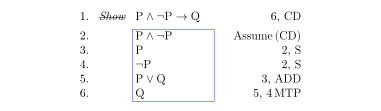
\includegraphics{b19aa63a56b0763796b01ccf0de48f7a89952148.pdf}

The following theorems are known as the \emph{paradoxes of material
implication}:

\renewcommand\labelitemi{$\oddorevenarrow$}

\phantomsection\label{almar1}
\marginnote{\begin{footnotesize}

\begin{itemize}
\tightlist
\item
  law of denying the antecedent
\end{itemize}

\end{footnotesize}}

\begin{equation}\phantomsection\label{eq-modal-t18}{
\class{alref}{\cssId{alref1}{}}\lnot \mathrm{P}\to(\mathrm{P}\to \mathrm{Q})\tag*{(T18)}
}\end{equation}

\vspace{-2\parskip}

\phantomsection\label{almar2}
\marginnote{\begin{footnotesize}

\begin{itemize}
\tightlist
\item
  law of affirming the consequent
\end{itemize}

\end{footnotesize}}

\begin{equation}\phantomsection\label{eq-modal-t2}{
\class{alref}{\cssId{alref2}{}}\mathrm{Q}\to(\mathrm{P}\to \mathrm{Q})\tag*{(T2)}
}\end{equation}

\vspace{-2\parskip}

\phantomsection\label{almar3}
\marginnote{\begin{footnotesize}

\begin{itemize}
\tightlist
\item
  conditional excluded middle
\end{itemize}

\end{footnotesize}}

\begin{equation}\phantomsection\label{eq-modal-t58}{
\class{alref}{\cssId{alref3}{}}(\mathrm{P}\to \mathrm{Q})\lor(\mathrm{Q}\to\lnot \mathrm{Q})\tag*{(T58)}
}\end{equation}

\vspace{-2\parskip}

\phantomsection\label{almar4}
\marginnote{\begin{footnotesize}

\begin{itemize}
\tightlist
\item
  Consequentia Mirabilis, ``admirable consequence'' {[}Cantor's
  \(\Delta\)?{]}
\end{itemize}

\end{footnotesize}}

\begin{equation}\phantomsection\label{eq-modal-t114}{
\class{alref}{\cssId{alref4}{}}(\lnot \mathrm{P}\to \mathrm{P})\to \mathrm{P}\tag*{(T114)}
}\end{equation}

\vspace{-1\parskip}

C. I. Lewis investigated modal logic in order to find a stricter form of
the conditional which would not result in such paradoxes. Lewis defined
\emph{strict implication} \(\mathrm{P}\Rightarrow \mathrm{Q}\) (read
``\(\mathrm{P}\) \emph{strictly implies} \(\mathrm{Q}\)'') by combining
modality with the truth-functional conditional: \[
\mathrm{P}\Rightarrow \mathrm{Q}\quad:=\quad\Box(\mathrm{P}\land\lnot \mathrm{Q}),
\] or alternatively, \[
\mathrm{P}\Rightarrow \mathrm{Q}\quad:=\quad\Box(\mathrm{P}\to \mathrm{Q}).
\]

The notion of strict implication was characterized by such axioms as:

The philosopher Leibniz (1646--1716) explicitly invoked that language of
possible worlds to explain the difference between necessary and
contingent truths. What is logically or necessarily true are those
truths truth in \emph{all} possible worlds, whereas a contingent truth
is one that is true in \emph{some} possible worlds.

Drawing upon this logical connection between universal and existential
quantification and the modal notions of necessity and possibility, we
obtain a modal version of the classical Aristotelian Square of
Opposition and the duality of modal laws known as the laws of modal
negation.

\begin{figure*}

\centering{

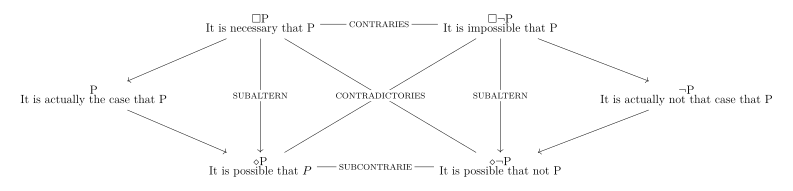
\includegraphics{d4b4d0178cfadc8c81925a3403484e4cbdf83fd6.pdf}

}

\caption{\label{fig-modal-aristotelian-diamond-1}\textsc{An Aristotelian
Diamond of Opposition}}

\end{figure*}%

In the modern development of modal logic, logicians noticed that a host
other phenomena---such as deontic notions of obligation and
permissibility, epistemic notions of knowledge and belief, as well as
temporal operators---share these logical relations and hence can be
represented as modal logics.

In \emph{deontic logic}, \(\Box\) is read ``it is morally obligatory
that'' and \({\Large\diamond}\) is read ``it is morally permissible
that''. Kant's maxim that ``ought implies can'', that is, whatever is
obligatory is permissible, is captured by modal axiom
\hyperref[eq-modal-axiom-D]{(\textbf{D})}:
\begin{equation}\phantomsection\label{eq-modal-axiom-D}{
\Box \mathrm{P} \to{\Large\diamond} \mathrm{P}.\tag*{(\textbf{D})}
}\end{equation}

In \emph{epistemic logic}, \(\Box\) is read for some subject \(S\) ``it
is known that'' and \({\Large\diamond}\) is read ``it is believed
that''. Some modal axioms for epistemic logic that have been considered
include:

\vspace{-2\parskip}
\renewcommand\labelitemi{$\oddorevenarrow$}

\phantomsection\label{almar5}
\marginnote{\begin{footnotesize}

\begin{itemize}
\tightlist
\item
  logical omniscience
\end{itemize}

\end{footnotesize}}

\begin{equation}\phantomsection\label{eq-modal-axiom-K}{
\class{alref}{\cssId{alref5}{}}\Box(\mathrm{P}\to \mathrm{Q})\to(\Box \mathrm{P}\to\Box \mathrm{Q})\tag*{(\textbf{K})}
}\end{equation}

\vspace{-2\parskip}

\phantomsection\label{almar6}
\marginnote{\begin{footnotesize}

\begin{itemize}
\tightlist
\item
  law of affirming the consequent
\end{itemize}

\end{footnotesize}}

\begin{equation}\phantomsection\label{eq-modal-axiom-T-2}{
\class{alref}{\cssId{alref6}{}}\Box \mathrm{P}\to \mathrm{P}\tag*{(\textbf{T})}
}\end{equation}

\vspace{-2\parskip}

\phantomsection\label{almar7}
\marginnote{\begin{footnotesize}

\begin{itemize}
\tightlist
\item
  law of affirming the consequent
\end{itemize}

\end{footnotesize}}

\begin{equation}\phantomsection\label{eq-modal-axiom-4}{
\class{alref}{\cssId{alref7}{}}\Box \mathrm{P}\to\Box\Box \mathrm{P}\tag*{(\textbf{4})}
}\end{equation}

\vspace{-2\parskip}

\phantomsection\label{almar8}
\marginnote{\begin{footnotesize}

\begin{itemize}
\tightlist
\item
  law of affirming the consequent
\end{itemize}

\end{footnotesize}}

\begin{equation}\phantomsection\label{eq-modal-axiom-E}{
\class{alref}{\cssId{alref8}{}}\lnot\Box \mathrm{P}\to\Box\lnot\Box \mathrm{P}\tag*{(\textbf{E})}
}\end{equation}

\vspace{-1\parskip}

The axiom \hyperref[eq-modal-axiom-K]{(\textbf{K})} expresses logical
omniscience insofar as this axiom requires that the knowledge of an
agent is closed under \emph{modus ponens}; and hence such knowers know
all the logical consequences of their knowledge.

Axiom \hyperref[eq-modal-axiom-T-2]{(\textbf{T})} states the truism that
whatever is known is true. Notice that this axiom would be too strong
for deontic logic insofar as an action's being obligatory doesn't imply
that the agent actually performs that action.

Axiom \hyperref[eq-modal-axiom-4]{(\textbf{4})} expresses a high degree
of \emph{positive introspective knowledge}: if someone knows P, then she
knows that she knows that \(\mathrm{P}\). Axiom
\hyperref[eq-modal-axiom-E]{(\textbf{E})} on the other hand, expresses a
high degree of \emph{negative} introspective knowledge: if someone
doesn't know that \(\mathrm{P}\), then he knows he doesn't know
\(\mathrm{P}\). This axiom is contrary to the experience of Socrates: as
the gadfly of Athens, Socrates found through his questioning that many
of his fellow Athenians did not know what they were talking about but
also didn't know that they didn't know. The gadfly of Athens believed
his vocation was to sting his fellow Athenians into the awareness they
were own ignorance, a service for which they did not always show
adequate appreciation.

The \emph{temporal logic} or Diodorian temporal logic was studied by the
logician A. N. Prior (1914--1969). To model temporal language, we
introduce a pair of modal operators for the future and a pair of modal
operators for the past.

\begin{longtable}[]{@{}
  >{\centering\arraybackslash}p{(\columnwidth - 2\tabcolsep) * \real{0.1200}}
  >{\raggedright\arraybackslash}p{(\columnwidth - 2\tabcolsep) * \real{0.8800}}@{}}
\toprule\noalign{}
\endhead
\bottomrule\noalign{}
\endlastfoot
\(\color{green}\Box\) & It {\color{green} \emph{is always going}}
{[}i.e., in \emph{all} futures{]} to be the case that \\
\(\color{green}{\Large\diamond}\) & It {\color{green}
\emph{will}\textgreater{}} {[}i.e., in \emph{some} future{]} be the case
that \\
\(\color{red}\Box\) & It {\color{red} \emph{has always been}} {[}i.e.,
in \emph{all} pasts{]} the case that \\
\(\color{red}{\Large\diamond}\) & It {\color{red} \emph{was once}{]}}
{[}i.e., in \emph{some} past or \emph{``once upon a time''}{]} the case
that \\
\end{longtable}

The axioms for minimal tense logic include version of Axiom
\hyperref[eq-modal-axiom-K]{(\textbf{K})} for the two necessity
operators: \begin{align*}
&{\color{red}\Box}(\varphi\to\psi)\to({\color{red}\Box}\varphi\to{\color{red}\Box}\psi)
&\begin{aligned}\text{\textit{Whatever has always followed from what always has been,}}\\\text{\textit{always has been.}}\end{aligned}&
\tag*{(K${\color{red}\Box}$)}\\\\
&{\color{green}\Box}(\varphi\to\psi)\to({\color{green}\Box}\varphi\to{\color{green}\Box}\psi)
&\begin{aligned}\text{\textit{Whatever will always follow from what always will be,}}\\\text{\textit{always will be.}}\end{aligned}&
\tag*{(K${\color{green}\Box}$)}
\end{align*}

It also contains two axioms concerning the interaction of the past and
future that has the form of the so-called Brouwersche axiom with
alternating valences: \begin{align*}
\tag*{(B${\color{green}\Box}{\color{red}{\Large\diamond}}$)}
&\varphi\to{\color{green}\Box}{\color{red}{\Large\diamond}}\varphi
&\text{\textit{What is, will always have been}}\\
\tag*{(B${\color{red}\Box}{\color{green}{\Large\diamond}}$)}
&\varphi\to{\color{red}\Box}{\color{green}{\Large\diamond}}\varphi
&\text{\textit{What is, has always been going to happen}}\\
\end{align*}

The Brouwersche \hyperref[eq-modal-axiom-B]{(\textbf{B})} axiom was
so-named by the logician Oskar Becker (Becker
1930)\marginpar{\begin{footnotesize}
\begin{CSLReferences}{2}{0}
\bibitem[\citeproctext]{ref-Becker1930Logik}
Becker, Oskar. 1930. Zur logik der modalit{ä}ten.
\end{CSLReferences}
\vspace{2mm}\par\end{footnotesize}}
after the charismatic Dutch mathematician L. E. J. Brouwer (1881--1966),
who championed a philosophy of mathematics known as \emph{intuitionism}.
It happens that when the \({\Large\diamond}\) can be paraphrased as
\({\Large\diamond}\lnot{\Large\diamond}\), the resulting axiom has the
form of the acceptable form of double negation in intuitionistic logic:
\begin{equation}\phantomsection\label{eq-modal-axiom-B}{
\varphi\to\lnot{\Large\diamond}\lnot{\Large\diamond}\varphi\tag*{(\textbf{B})}
}\end{equation}

\marginnote{\begin{footnotesize}

\begin{tcolorbox}[enhanced jigsaw, breakable, bottomtitle=1mm, colback=white, bottomrule=.15mm, opacitybacktitle=0.6, rightrule=.15mm, leftrule=.75mm, left=2mm, colbacktitle=quarto-callout-tip-color!10!white, colframe=quarto-callout-tip-color-frame, title=\textcolor{quarto-callout-tip-color}{\faLightbulb}\hspace{0.5em}{A Classical Theorem, but in Intuitionism}, toptitle=1mm, opacityback=0, coltitle=black, titlerule=0mm, toprule=.15mm, arc=.35mm]

\textbf{Theorem.} There exist two irrational numbers \(x\) and \(y\)
such that \(x^y\) is irrational.

\begin{proof}
Consider \[
\sqrt{2}^{\left(\sqrt{2}^{\sqrt{2}}\right)}
=\sqrt{2}^{\left(\sqrt{2}\cdot\sqrt{2}\right)}
=\sqrt{2}^2=2,
\] which is rational.

\renewcommand\labelitemi{\labelitemito}

The number \(\sqrt{2}^{\sqrt{2}}\) is either rational or irrational.

\begin{itemize}
\tightlist
\item
  If it's rational, then \(x=y=\sqrt{2}\) are both irrational yet
  \(x^y\) is rational.
\item
  If \(\sqrt{2}^{\sqrt{2}}\) is irrational, then
  \(x=\sqrt{2}^{\sqrt{2}}\) and \(y=\sqrt{2}\) are both irrational and
  \(x^y\) is rational.
\end{itemize}

Either way, there exists \(x\) and \(y\) such that \(x^y\) is rational.
\end{proof}

Intuitionists reject this classical argument by separation of cases
because it does not actually construct the numbers \(x\) and \(y\) such
that \(xy\) is irrational. The idea behind intuitionistic logic is that
the connectives are reinterpreted as involving a kind of provability.

In case you're curious, it is actually known that
\(\sqrt{2}^{\sqrt{2}}\) is irrational, due to the
\href{https://en.wikipedia.org/wiki/Gelfond\%E2\%80\%93Schneider_theorem}{Gelfond--Schneider
theorem} which verifies that it usually take significantly more effort
to convince an intuitionistic mathematicians than a classical one.

\end{tcolorbox}

\end{footnotesize}}

According to intuitionism, mathematical objects do not exist as eternal
Platonic objects but are constructions in intuition. Intuitionists read
the propositional connectives as involving not merely truth, but proof,
and so they rejected such classical forms of reasoning as \emph{reductio
ad absurdum} and theorems such as the \emph{law of excluded middle.}
Intuitionists reject the following mathematical proof.

Around the 1970s it was noticed that the famous incompleteness theorems
(Gödel
1931)\marginpar{\begin{footnotesize}
\begin{CSLReferences}{2}{0}
\bibitem[\citeproctext]{ref-Godel1931Incomepleteness}
Gödel, Kurt. 1931. {Ü}ber formal unentscheidbare s{ä}tze der principia
mathematica und verwandter systeme i. \emph{Monatshefte f{ü}r Mathematik
Und Physik} 38. 173--198.
\end{CSLReferences}
\vspace{2mm}\par\end{footnotesize}}
were propositional in character and that their logic could be captured
in propositional modal logic. These modal provability logics added to
Axiom \hyperref[eq-modal-axiom-K]{(\textbf{K})} the following axiom,
known as the Gödel-Löb axiom or also the well-ordering axiom.
\begin{equation}\phantomsection\label{eq-modal-axiom-W}{
\Box(\Box\varphi\to\varphi)\to\Box\varphi\tag*{(\textbf{W})}
}\end{equation}

\emph{Modal Provability Logics} proliferated from the 1950s--1970s, but
the genesis of the idea goes back to a short note of Gödel
(1933)\marginpar{\begin{footnotesize}
\begin{CSLReferences}{2}{0}
\bibitem[\citeproctext]{ref-Godel1933}
Gödel, Kurt. 1933. Eine interpretation des intuitionistischen
aussagenkalküls. \emph{Ergebnisse Eines Mathematischen Kolloquiums} 4.
39--40.
\end{CSLReferences}
\vspace{2mm}\par\end{footnotesize}}
in which he noted that intuitionistic truth is defined in terms of proof
since provability is a kind of necessity. The above axiom can be read as
a kind of soundness theorem.

\renewcommand\labelitemi{}

\begin{itemize}
\tightlist
\item
  \emph{if it is provable that \(\varphi\) being provable implies it is
  true, then \(\varphi\) is provable.}
\end{itemize}

\renewcommand\labelitemi{\labelitemito}

Later we will show how to use a modal provability logic to exhibit the
propositional logic of key parts of Gödel's First and Second
Incompleteness Theorems.

In contemporary logic, modal logic has grown beyond these philosophical
origins and is at the interface of a number of disciplines including the
studies information flow and dynamics, game theory, and computability.

\subsubsection*{Exercises}\label{exercises}
\addcontentsline{toc}{subsubsection}{Exercises}

\begin{enumerate}
\def\labelenumi{(\arabic{enumi})}
\tightlist
\item
  Symbolize the following modal arguments.

  \begin{enumerate}
  \def\labelenumii{(\Alph{enumii})}
  \tightlist
  \item
    Eratosthenes must either be in Syene or Alexandria. Eratosthenes
    cannot be in Syene. Therefore, Eratosthenes must be in Alexandria.
  \item
    Assume that justice can be defined as paying your debts and telling
    the truth. Then it is \emph{morally obligatory} for Cephalus to
    comply to a madman's request that Cephalus return a borrowed sword
    and that Cephalus tell the truth about the whereabouts of a friend
    whom the madman wants to kill with the sword. However, if this act
    is \emph{morally obligatory}, then it is \emph{morally permissible}.
    However, it is \emph{morally impermissible} (or \emph{morally
    forbidden}) for Cephalus to comply. So it isn't \emph{morally
    obligatory} for Cephalus to comply. Justice, therefore, cannot be
    defined as paying your debts and telling the truth.
  \item
    It is conceivable that I am having experiences qualitatively
    identical to those I am having now on the supposition that I am
    being deceived by an evil genius. If that is conceivable, then I do
    not have indubitable knowledge that the external world exists.
  \end{enumerate}
\item
  Johan van Benthem (Van Benthem 2010:
  12)\marginpar{\begin{footnotesize}
\begin{CSLReferences}{2}{0}
\bibitem[\citeproctext]{ref-VanBenthem2010}
Van Benthem, Johan. 2010. \emph{Modal logic for open minds}. Stanford,
CA: Centre for the Study of Language \& Information.
\end{CSLReferences}
\vspace{2mm}\par\end{footnotesize}}
  was asked to symbolize the philosophical claim that ``nothing is
  absolutely relative''. He came up with the following:
  \[\lnot\Box({\Large\diamond}\varphi\land{\Large\diamond}\lnot\varphi).\]
  Use familiar equivalences from propositional logic and the modal
  negation laws to show that this symbolization is equivalent to
\end{enumerate}

\renewcommand\labelitemi{$\oddorevenarrow$}

\phantomsection\label{almar9}
\marginnote{\begin{footnotesize}

\begin{itemize}
\tightlist
\item
  \emph{McKinsey's Axiom}
\end{itemize}

\end{footnotesize}}

\begin{equation}\phantomsection\label{eq-modal-axiom-M}{
\class{alref}{\cssId{alref9}{}}
\Box{\Large\diamond}\varphi\to{\Large\diamond}\Box\varphi\tag*{(\textbf{M})}
}\end{equation}

\renewcommand\labelitemi{\labelitemito}

\begin{enumerate}
\def\labelenumi{(\arabic{enumi})}
\setcounter{enumi}{2}
\item
  Match the following symbolizations with the best corresponding
  translation below.

  \begin{longtable}[]{@{}
    >{\raggedleft\arraybackslash}p{(\columnwidth - 2\tabcolsep) * \real{0.2500}}
    >{\raggedright\arraybackslash}p{(\columnwidth - 2\tabcolsep) * \real{0.7500}}@{}}
  \toprule\noalign{}
  \begin{minipage}[b]{\linewidth}\raggedleft
  symbolization
  \end{minipage} & \begin{minipage}[b]{\linewidth}\raggedright
  translation
  \end{minipage} \\
  \midrule\noalign{}
  \endhead
  \bottomrule\noalign{}
  \endlastfoot
  \({\color{red}{\Large\diamond}\Box}\mathrm{P}\) & \emph{It was always
  the case that it will sometime be the case that} \(\mathrm{P}\). \\
  \({\color{green}{\Large\diamond}}\mathrm{P}\to{\color{green}{\Large\diamond}}\mathrm{P}\)
  & \emph{It will sometime be the case that it was once the case that}
  \(\mathrm{P}\). \\
  \({\color{red}\Box}{\color{green}{\Large\diamond}}\mathrm{P}\) &
  \emph{Whatever will always be, will be.} \\
  \({\color{green}{\Large\diamond}}{\color{red}{\Large\diamond}}\mathrm{P}\)
  & \emph{Once upon a time, it was always the case that}
  \(\mathrm{P}\). \\
  \end{longtable}
\end{enumerate}

\renewcommand\caption[1][]{\captionto{#1}}

\section{}\label{section}

\section{}\label{section-1}

\section{}\label{section-2}

\section{}\label{section-3}

\section{}\label{section-4}

\section{\texorpdfstring{\textsc{Possible World
Semantics}}{Possible World Semantics}}\label{possible-world-semantics}

The Leibnizian idea of characterizing necessity and possibility in terms
of truth in all or some possible worlds was given an elegant
formalization by (Kripke 1959;
1963)\marginpar{\begin{footnotesize}
\begin{CSLReferences}{2}{0}
\bibitem[\citeproctext]{ref-Kripke1959}
Kripke, Saul. 1959. A completeness theorem in modal logic. \emph{Journal
of Symbolic Logic} 24(1). 1--14. DOI:
https://doi.org/\href{https://doi.org/10.2307/2964568}{10.2307/2964568}
\end{CSLReferences}
\vspace{2mm}\par\end{footnotesize}}\marginpar{\begin{footnotesize}
\begin{CSLReferences}{2}{0}
\bibitem[\citeproctext]{ref-Kripke1963}
Kripke, Saul. 1963. Semantical analysis of modal logic i normal modal
propositional calculi. \emph{Mathematical Logic Quarterly} 9(5-6).
67--96. DOI:
https://doi.org/\url{https://doi.org/10.1002/malq.19630090502}
\end{CSLReferences}
\vspace{2mm}\par\end{footnotesize}}
when he was only a teenager. According to Leibniz, a sentence is
\emph{necessary} if it is true in \emph{every} possible world, and a
sentence is \emph{possible} if it is true is \emph{some} possible world.
Kripke showed that by placing very natural conditions on a relation of
\emph{relative possibility} or \emph{accessibility} on a set of possible
worlds, the various systems of modal logic could be validated.

Intuitively, a possible world tells us for each sentence letter whether
it is true or false in that world. Stripping away inessentials, we can
represent a possible world by a subset of sentence letters. A
\emph{modal structure} \(\mathbb{M}\) is an ordered triple
\(\langle W, R,\alpha \rangle\), where \(W\) is a set\sidenote{\footnotesize set-theoretic
  size issues‽} of possible worlds, \(R\subseteq W\times W\) is a
relation known as the \emph{accessibility relation} or the
\emph{relative possibility relation}, and \(\alpha\) is a distinguished
element of \emph{W} known as the \emph{actual world}

We can exhaustively characterize the notion of \[\beta \vDash \varphi,\]
the \emph{truth of a sentence in a possible world} \(\beta\), by

\begin{enumerate}
\def\labelenumi{(\arabic{enumi})}
\setcounter{enumi}{3}
\item
  If \(\varphi\) is a sentence letter S, then \[
  \beta\vDash S \iff S\in\beta,
  \] i.e.~\(S\) is a member of \(\beta\);
\item
  If \(\varphi\) is \(\psi\), then \[
  \beta\vDash \neg\psi \iff \beta\not\vDash\psi,
  \] i.e., it is not the case that \(\beta\vDash\psi\);
\item
  \begin{enumerate}
  \def\labelenumii{(\alph{enumii})}
  \item
    If \(\varphi\) is \((\psi\land\chi)\), then \[
    \beta\vDash (\psi\land\chi) \iff \beta\vDash\psi \mathrel{\&} \beta\vDash\chi,
    \] i.e., both \(\beta\vDash\psi\) and \(\beta\vDash\chi\);
  \item
    If \(\varphi\) is \((\psi\lor\chi)\), then \[
    \beta\vDash (\psi\lor\chi) \iff \beta\vDash\psi \mathrel{\|} \beta\vDash\chi,
    \] i.e., either \(\beta\vDash\psi\) or \(\beta\vDash\chi\), or both;
  \item
    If \(\varphi\) is \((\psi\to\chi)\), then \[
    \beta\vDash (\psi\to\chi) \iff \beta\vDash\psi\implies\chi,
    \] i.e., if \(\beta\vDash\psi\) then \(\beta\vDash\chi\), or either
    \(\beta\not\vDash\psi\) or \(\beta\vDash\chi\) ‽;
  \item
    If \(\varphi\) is \((\psi\leftrightarrow\chi)\), then \[
    \beta\vDash (\psi\leftrightarrow\chi) \iff \beta\vDash\psi\iff\chi,
    \] i.e., \(\beta\vDash\psi\) if and only if \(\beta\vDash\chi\);
  \end{enumerate}
\end{enumerate}

Finally, the law clause gives the Leibnizian truth conditions for
necessity and possibility:

\begin{enumerate}
\def\labelenumi{(\arabic{enumi})}
\setcounter{enumi}{6}
\item
  \begin{enumerate}
  \def\labelenumii{(\alph{enumii})}
  \item
    If \(\varphi\) is \(\Box\psi\), then \[
    \beta\vDash \Box\psi \iff \forall \gamma\in W.\, \beta\mathrel{R}\gamma \implies \beta\vDash\psi,
    \] i.e., \(\psi\) is true in \emph{all} possible worlds \(\gamma\),
    possible-relative to \(\beta\);
  \item
    If \(\varphi\) is \({\Large\diamond}\psi\), then \[
    \beta\vDash {\Large\diamond}\psi \iff \exists \gamma\in W.\, \beta\mathrel{R}\gamma \implies \beta\vDash\psi,
    \] i.e., \(\psi\) is true in some possible worlds \(\gamma\),
    possible-relative to \(\beta\);
  \end{enumerate}
\end{enumerate}

This completes the definition of truth in a model for modal
propositional logic. Using this definition of truth, we can now define
what it means for a sentence to be \emph{semantically valid}: \[
\vDash\varphi\text{ (i.e., }\varphi\text{ is semantically valid)} \iff \forall\alpha\in W.\, \alpha\vDash\varphi.
\]

Next, we obtain different systems of modal logic when various conditions
are placed on the accessibility or relative possibility relation R. We
say that a relation \(R\) is a \emph{series} if \(R\) is serial; \(R\)
is a \emph{reflexivity} if \(R\) is totally reflexive; \(R\) is a
\emph{similarity} if \(R\) is totally reflexive and symmetric; \(R\) is
a \emph{partial ordering} if \(R\) is totally reflexive and transitive;
\(R\) is an \emph{equivalence relation} if \(R\) is totally reflexive
and euclidean. It turns out that the axioms of modal logic discussed
above are validated when natural conditions are imposed on the
accessibility or relative possibility relation \(R\).

\begin{longtable}[]{@{}
  >{\centering\arraybackslash}p{(\columnwidth - 6\tabcolsep) * \real{0.1000}}
  >{\raggedright\arraybackslash}p{(\columnwidth - 6\tabcolsep) * \real{0.2000}}
  >{\raggedright\arraybackslash}p{(\columnwidth - 6\tabcolsep) * \real{0.2000}}
  >{\raggedright\arraybackslash}p{(\columnwidth - 6\tabcolsep) * \real{0.5000}}@{}}
\caption{Properties of
Accessibility}\label{tbl-properties-of-accessibility}\tabularnewline
\toprule\noalign{}
\endfirsthead
\endhead
\bottomrule\noalign{}
\endlastfoot
\textbf{D} &
\({\small\square} \varphi \rightarrow {\Large\diamond} \varphi\) &
serial &
\(\forall \alpha.\,\exists \beta.\, \alpha \mathbin{R} \beta\) \\
\textbf{T} & \({\small\square} \varphi \rightarrow \varphi\) & reflexive
& \(\forall \alpha.\,\alpha \mathbin{R} \alpha\) \\
\textbf{B} & \(\varphi \rightarrow \square {\Large\diamond} \varphi\) &
symmetric &
\(\forall \alpha.\, \forall \beta.\, (\alpha \mathbin{R} \beta \Rightarrow \beta \mathbin{R} \alpha)\) \\
\textbf{4} & \(\square \varphi \rightarrow \square \square \varphi\) &
transitive &
\(\forall \alpha \forall \beta .\, \forall \gamma.\, (\alpha \mathbin{R} \beta \;\&\; \beta \mathbin{R} \gamma \Rightarrow \alpha \mathbin{R} \gamma)\) \\
\textbf{5} &
\({\Large\diamond} \varphi \rightarrow \square {\Large\diamond} \varphi\)
& euclidean &
\(\forall \alpha.\, \forall \beta.\, \forall \gamma.\, (\alpha \mathbin{R} \beta \;\&\; \alpha \mathbin{R} \gamma \Rightarrow \beta \mathbin{R} \gamma)\) \\
\end{longtable}

Systems of modal logic are \emph{normal} when everything derivable from
necessary truths is itself necessary. This will be the case if the rule
of \emph{modus ponens} and axiom
\hyperref[eq-modal-axiom-K-2]{(\textbf{K})} are valid:
\begin{equation}\phantomsection\label{eq-modal-axiom-K-2}{
\Box(\mathrm{P}\to \mathrm{Q})\to(\Box \mathrm{P}\to\Box \mathrm{Q}).\tag*{(\textbf{K})}
}\end{equation}

Axiom \textbf{K} expresses the intuition that \emph{necessary truths
imply only necessary truths}.

We can conveniently summarize the above systems of modal logic in a
chart. The various modal systems can be characterized by the axioms that
are valid in them. The smallest normal modal logic system \textbf{K}
contains axiom \textbf{K}. The four most famous modal logics are system
(T) named after the Gödel--Feyes--von Wright modal logic to model
tautologies, system \textbf{S4} and \textbf{S5}, named after C. I.
Lewis's axioms for strict implications, and the unduly neglected
Brouwersche system \textbf{B}, named by Becker after the intuitionist L.
E. J. Brouwer due to the characteristic axiom's similarity to
intuitionistic double negation. All these systems contain \textbf{K} and
\textbf{T}. The system \textbf{D} is a weaker system than \textbf{T},
containing axioms \textbf{K} and \textbf{D}, is named for deontic logic.

Notice that relationships of containment among the modal systems follow
from the logic of relations. Axiom \textbf{B} requires that R be
symmetric and \textbf{4} requires that R be transitive. System
\textbf{S5} with axioms \textbf{T} and \textbf{E} require R to be an
equivalence relation (i.e., reflexive, symmetric, and transitive);
hence, \textbf{S5} could also be specified by requiring axioms
\textbf{T}, \textbf{4}, and \textbf{B} to be valid. Therefore,
\textbf{S5} contains \textbf{S4} and \textbf{B}, neither of which
contains the other. Systems \textbf{S5}, \textbf{S4} and \textbf{B} all
contain system \textbf{T}, which contains \textbf{D}.

A convenient way of describing these modal logics is by their
\emph{Lemmon code} listing the axioms valid in them. For example,
\(\mathbf{S5} = \mathbf{KTE} = \mathbf{KT4B} = \mathbf{KD4B}\). We can
represent these containment relations in a diagram in which downward
paths represent containment.

\begin{longtable}[]{@{}
  >{\centering\arraybackslash}p{(\columnwidth - 10\tabcolsep) * \real{0.1000}}
  >{\raggedright\arraybackslash}p{(\columnwidth - 10\tabcolsep) * \real{0.2300}}
  >{\centering\arraybackslash}p{(\columnwidth - 10\tabcolsep) * \real{0.1000}}
  >{\raggedright\arraybackslash}p{(\columnwidth - 10\tabcolsep) * \real{0.2300}}
  >{\centering\arraybackslash}p{(\columnwidth - 10\tabcolsep) * \real{0.1000}}
  >{\raggedright\arraybackslash}p{(\columnwidth - 10\tabcolsep) * \real{0.2300}}@{}}
\caption{Modal Axioms and
Accessibility}\label{tbl-modal-axioms-and-accessibility}\tabularnewline
\toprule\noalign{}
\endfirsthead
\endhead
\bottomrule\noalign{}
\endlastfoot
\textbf{D} & Deontic Logic & \textbf{D} &
\({\small\square} P \rightarrow {\Large\diamond} P\) & \textbf{KD} &
seriality \\
\textbf{T} & Gödel-Feys-von Wright Tautology & \textbf{T} &
\({\small\square} P \rightarrow P\) & \textbf{KT} & reflexivity \\
\textbf{B} & Brouwersche System & \textbf{B} &
\(P \rightarrow \square {\Large\diamond} P\) & \textbf{KTB} &
similarity \\
\textbf{S4} & Lewis' Strict Implication System 4 & \textbf{4} &
\(\square P \rightarrow \square \square P\) & \textbf{KT4} & partial
ordering \\
\textbf{S5} & Lewis' Strict Implication System 5 & \textbf{E} &
\({\Large\diamond} P \rightarrow \square {\Large\diamond} P\) &
\textbf{KTE} & equivalence relation \\
\end{longtable}

\begin{marginfigure}

\centering{

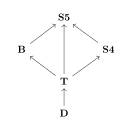
\includegraphics{a1aa6cce761cea6d0a8bc1e6ee85e3bd094d5dc9.pdf}

}

\caption{\label{fig-logical-containment-of-the-modal-systems}Logical
Containment of the Modal Systems}

\end{marginfigure}%

Various deontic modal systems can also be characterized by their axioms
(\emph{Lemmon code}).

\begin{longtable}[]{@{}
  >{\centering\arraybackslash}p{(\columnwidth - 6\tabcolsep) * \real{0.2000}}
  >{\raggedright\arraybackslash}p{(\columnwidth - 6\tabcolsep) * \real{0.3000}}
  >{\raggedright\arraybackslash}p{(\columnwidth - 6\tabcolsep) * \real{0.2000}}
  >{\raggedright\arraybackslash}p{(\columnwidth - 6\tabcolsep) * \real{0.3000}}@{}}
\caption{Lemmon Codes for Deontic Modal
Systems}\label{tbl-lemmon-codes-for-deontic-modal-systems}\tabularnewline
\toprule\noalign{}
\endfirsthead
\endhead
\bottomrule\noalign{}
\endlastfoot
System \textbf{T} & \textbf{KT} & Deontic \textbf{D} & \textbf{KD} \\
System \textbf{B} & \textbf{KTB} & & \\
System \textbf{S4} & \textbf{KT4} & Deontic \textbf{S4} &
\textbf{KD4} \\
System \textbf{S5} & \textbf{KTE} = \textbf{KT4B} = \textbf{KD4B} & & \\
\end{longtable}

The logical relationships among the above systems of modal logic can be
set forth in a diagram (due to Krister Segerberg who omits \textbf{KD5}
and \textbf{K45}). As before, a modal logic is included in another if it
is connected to it, directly or indirectly, by an upward path. The
second diagram is a more elaborate \textsc{Picassos' Electric Chair}
that includes deontic modal logics.

\clearpage

\begin{figure*}[H]

\centering{

\begin{figure*}[H]

\begin{minipage}{0.50\linewidth}
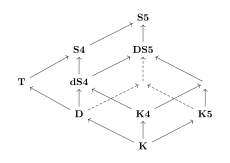
\includegraphics{becb4b6f90dba6e7b9ba11cb913e86bf19f4d746.pdf}\end{minipage}%
%
\begin{minipage}{0.50\linewidth}
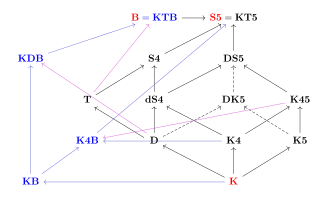
\includegraphics{8c9cdf2bc4708274af4c6f18832953666a027fdc.pdf}\end{minipage}%

\end{figure*}%

}

\caption{\label{fig-picassos-hasse-diagrams}Hasse--Picassos Diagrams for
Systems of Modal Logic}

\end{figure*}%

One way to visualize how the conditions on the accessibility relation
validate their respective axioms is using the definitions of
`\(\small\square\)' and \(\LARGE\diamond\) in terms of possible worlds
and use directed graphs from Chapter IV to represent the accessibility
relation \(\mathbin{R}\). Here the accessibility relation
\(\alpha\mathbin{R}\beta\) (read ``\(\beta\) is possible relative to
\(\alpha\)'''' or ``\(\beta\) is accessible to \(\alpha\)'') is
represented by an arrow from a circle representing possible world
\(\alpha\) to a circle representing possible world \(\beta\).

\begin{marginfigure}

\centering{

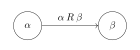
\includegraphics{bd366b3b4f44f34c8e8add34c09ad50163e16ffa.pdf}

}

\caption{\label{fig-accessibility-represented-by-directed-graphs}Accessibility
Represented by Directed Graphs}

\end{marginfigure}%

We can, using the directed graphs from the theory of relations,
translate properties of accessibility relations into geometric
properties of directed graphs. Symmetry, for example, requires that all
accessibility arrows are double arrows. Reflexivity requires that every
world be accessible to itself and so every world has a loop, which is a
special case of a double arrow. Seriality requires that every world is a
tail of an arrow. Transitivity requires that for every indirect path of
accessibility from \(\alpha\) to \(\beta\) and from \(\beta\) to
\(\gamma\), there is a direct path from \(\alpha\) to \(\gamma\). Being
euclidean and serial is equivalent to being an equivalence relation,
that is, being reflexive, symmetric and transitive. Expressing
\(\mathbin{R}\) in terms of love and worlds in terms of persons, we have
the following intuitive translations:

\begin{longtable}[]{@{}
  >{\raggedright\arraybackslash}p{(\columnwidth - 4\tabcolsep) * \real{0.2000}}
  >{\raggedright\arraybackslash}p{(\columnwidth - 4\tabcolsep) * \real{0.3000}}
  >{\raggedright\arraybackslash}p{(\columnwidth - 4\tabcolsep) * \real{0.2000}}@{}}
\caption{Relational Properties of Directed
Graphs}\label{tbl-relational-properties-of-directed-graphs}\tabularnewline
\toprule\noalign{}
\endfirsthead
\endhead
\bottomrule\noalign{}
\endlastfoot
serial & \(\forall \alpha.\,\exists \beta.\, \alpha \mathbin{R} \beta\)
& Everyone is a lover. \\
reflexive & \(\forall \alpha.\,\alpha \mathbin{R} \alpha\) & Everyone is
a self-lover. \\
symmetric &
\(\forall \alpha.\, \forall \beta.\, (\alpha \mathbin{R} \beta \Rightarrow \beta \mathbin{R} \alpha)\)
& All love is requited; all love is mutual. \\
transitive &
\(\forall \alpha.\, \forall \beta .\, \forall \gamma.\, (\alpha \mathbin{R} \beta \;\&\; \beta \mathbin{R} \gamma \Rightarrow \alpha \mathbin{R} \gamma)\)
& Love is transitive. \\
euclidean &
\(\forall \alpha.\, \forall \beta.\, \forall \gamma.\, (\alpha \mathbin{R} \beta \;\&\; \alpha \mathbin{R} \gamma \Rightarrow \beta \mathbin{R} \gamma)\)
& All beloveds of the same lover, love each other and themselves. \\
\end{longtable}

Using the definition of truth in a modal system set forth above, we can
rigorously demonstrate that if R is transitive, then axiom \textbf{4} is
valid. This demonstration is carried out in the meta-language. We use
the symbols `\(\forall\)', `\(\exists\)', `\(\&\)', `\(\implies\)' and
`\(\in\)' in the meta-language for `all', `some', `and', `if\ldots{}
then', and `is an element of', respectively. Once the truth clauses are
unpacked, the logical demonstration is no more complicated than a
derivation in the theory of relations.

\phantom{a}

\begin{codelisting}

\caption{\label{lst-kaplan-transitivity-implies-validity-of-axiom-4}Kaplan
Semantic Derivation of Transitivity Validating Axiom 4}

\centering{

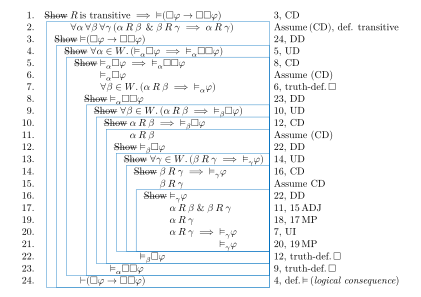
\includegraphics{7a1a22f066975e537e0d3785c6b7ea28e2823b0c.pdf}

}

\end{codelisting}%

\phantom{a}

The above semantic derivation can be visualized graphically to prove the
above result contrapositively. We will show that if
\[{\small\square}\varphi\to{\small\square}{\small\square}\varphi\] is
false, then the accessibility relation cannot be transitive. Axiom (4)
fails when its antecedent \(\varphi\) is true but its consequent
\({\small\square}\varphi\) is false in α. By modal negation,
\(\neg{\Large\diamond}{\Large\diamond}\varphi\) is equivalent to
\({\Large\diamond}{\Large\diamond}\neg\varphi\).

So both \({\small\square}\varphi\) and
\({\Large\diamond}{\Large\diamond}\neg\varphi\) are true in some
possible world \(\alpha\). Eliminating the first \({\Large\diamond}\),
we have that in some possible world \(\beta\) accessible to \(\alpha\)
(i.e.~\(\alpha\mathbin{R}\beta\)), \({\Large\diamond}\neg\varphi\) is
true. Applying the definition of truth for \({\LARGE\diamond}\) again,
we have that for some world \(\gamma\) accessible to \(\beta\)
(i.e.~\(\beta\mathbin{R}\gamma\)), \(\neg\varphi\) is true in
\(\gamma\). Notice that the transitivity of the accessibility relation
\(R\) would require that \(\gamma\) be accessible to \(\alpha\), which
would contradict that \({\small\square}\varphi\). The invalidity of
Axiom (\textbf{4}) implies the failure of the transitivity of the
accessibility relation \(R\). Stating this result contrapositively, if
the accessibility relation \(R\) is transitive, then axiom (\textbf{4})
is valid.

\begin{figure}[H]

\centering{

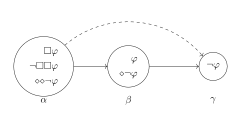
\includegraphics{5ed238651461db20668b3050b4c33e3735b0ab1a.pdf}

}

\caption{\label{fig-modal-kripke-worlds-diagram-transitivity-to-axiom-4}Kripke--Mar
Diagram for Transitivity of \(R\) Validating Axiom (4)}

\end{figure}%

The semantic demonstration together with the graphic proof using
directed graphs support one another in building our intuitions for modal
logic. The graphic proofs are satisfying because of their simplicity and
ability to make the critical step visually perspicuous. On the other
hand, the semantic proof is satisfying insofar as the explicit
definitions of \(\small\square\), \(\LARGE\diamond\), \(\vDash\) are
shown to work elegantly and precisely with our natural deduction systems
using the quantifier logic with UD, UI, EI, EG and the theory of
relations. We will use the directed graphs in the context of discovering
new axioms and the semantic proofs in the context of justifying that
these axioms correspond to imposing requirements on the accessibility
relation.

\subsection*{Exercises}\label{exercises-1}
\addcontentsline{toc}{subsection}{Exercises}

TODO\ldots{} too many graphics\ldots{} need some rest today\ldots{}

\bookmarksetup{startatroot}

\end{document}
